\documentclass[11pt]{article}
\usepackage[letterpaper,margin=1in]{geometry}
\usepackage{amsmath,amssymb,amsthm,graphicx,booktabs,microtype}
\usepackage[round]{natbib}
\usepackage[colorlinks=true,allcolors=blue]{hyperref}
\usepackage{placeins}
\newtheorem{proposition}{Proposition}
\newtheorem{theorem}[proposition]{Theorem}
\newcommand{\R}{\mathbb R}
\newcommand{\one}{\mathbf 1}
\newcommand{\norm}[1]{\lVert#1\rVert}
\newcommand{\E}{\mathcal E}
\DeclareMathOperator*{\argmin}{arg\,min}
\providecommand{\manuscriptversion}{unversioned}
\providecommand{\manuscriptbuildnumber}{NA}
\providecommand{\manuscriptcommit}{unknown}
\providecommand{\manuscriptbuilddatetime}{unknown}
\InputIfFileExists{build/manuscript_build_info.tex}{}{}
% Generated by check_focused_numbers.py; do not edit.
\newcommand{\numBoundedGraphs}{25}
\newcommand{\numStressWins}{23}
\newcommand{\numClassicalBefore}{3.451}
\newcommand{\numClassicalAfter}{0.245}
\newcommand{\numStressBefore}{2.264}
\newcommand{\numStressAfter}{0.164}
\newcommand{\numCoordLow}{4.60}
\newcommand{\numCoordHigh}{27.54}
\newcommand{\numRadiusGraphs}{1{,}216}
\newcommand{\numRadiusCandidates}{16{,}416}
\newcommand{\numRepairedGraphs}{74}
\newcommand{\numInputMatrices}{88}
\newcommand{\numRadiusStarts}{3{,}648}
\newcommand{\numCappedStarts}{25}
\newcommand{\numValidationPairs}{256}
\newcommand{\numGeodesicDiscrepancy}{5.16\times10^{-8}}
\newcommand{\numValidatedCoordinates}{16{,}928}
\newcommand{\numCoordinateDiscrepancy}{2.59\times10^{-12}}
\newcommand{\numGeodesicSaddlePath}{0.36}
\newcommand{\numGeodesicSaddleCoord}{80.38}
\newcommand{\numAmbientSaddlePath}{37.00}
\newcommand{\numAmbientSaddleCoord}{0.90}
\newcommand{\numFullInitializerCases}{84}
\newcommand{\numNeighborhoodSpreadMin}{8.05}
\newcommand{\numNeighborhoodSpreadMedian}{23.05}
\newcommand{\numNeighborhoodSpreadMax}{58.31}
\newcommand{\numNestedBase}{7.77}
\newcommand{\numNestedSameK}{9.23}
\newcommand{\numNestedSameFraction}{2.34}
\newcommand{\numClassicalPerturbation}{0.01888}
\newcommand{\numClassicalRandomFixed}{0.82}
\newcommand{\numStressPerturbation}{0.00031}
\newcommand{\numStressRandomFixed}{0.82}
\newcommand{\numProfiledCount}{6{,}080}
\newcommand{\numProfiledBelowHalf}{830}
\newcommand{\numProfiledBelowTenth}{475}
\newcommand{\numProfiledBelowThousandth}{262}
\newcommand{\numProfiledMedian}{1.028}
\newcommand{\numProfiledMinimum}{4.07\times10^{-10}}
\newcommand{\numFixedMinimum}{0.99339}
\newcommand{\numFixedMaximum}{1.02624}
\newcommand{\numPrimaryGraphs}{1{,}176}
\newcommand{\numProfiledImproved}{1{,}016}
\newcommand{\numProfiledWorsened}{76}
\newcommand{\numProfiledTied}{84}
\newcommand{\numFixedImproved}{1{,}075}
\newcommand{\numFixedWorsened}{17}
\newcommand{\numFixedTied}{84}
\newcommand{\numAmbientSaddleHorizontal}{35.24}
\newcommand{\numAmbientSaddleVertical}{0.03}
\newcommand{\numAmbientSaddleHeightOnly}{2.64}
\newcommand{\numAmbientParaboloidHorizontal}{23.66}
\newcommand{\numAmbientParaboloidVertical}{0.05}
\newcommand{\numAmbientParaboloidHeightOnly}{3.74}
\newcommand{\numGeodesicParaboloidHorizontal}{38.58}
\newcommand{\numGeodesicParaboloidVertical}{0.20}
\newcommand{\numGeodesicParaboloidHeightOnly}{3.74}
\newcommand{\numRetainedRouteDiscrepancy}{7.60\times10^{-15}}

\title{What Graph-Geodesic Embeddings Preserve:\\Path Fidelity, Scale, and Geometric Recovery}
\author{Pawel Gajer and Jacques Ravel}
\date{Author review draft, built \manuscriptbuilddatetime}
\begin{document}
\maketitle
\begin{abstract}
When observations lie on a curved or branching structure, distances along a
neighborhood graph can represent relationships that straight-line distances
in the observation space miss. Embedding the graph introduces a further
choice: should the drawing preserve distances between endpoints, or lengths
along the paths joining them? We examine what these criteria imply for
geometric recovery by comparing classical scaling, metric stress
multidimensional scaling (MDS), and edge-length refinement on sampled
paraboloids and saddles. Uniform geodesic bounds show that expanding
paraboloids approach a line metric after normalization, while saddles approach
a four-branch tree metric. Under an explicit sample-rank condition, the
saddle's classical-MDS limit spans three Euclidean dimensions even though the
limiting tree is intrinsically one-dimensional. Two controlled studies show
how this distinction enters finite-sample embeddings. Edge refinement improves
retained-path agreement under both MDS initializers throughout a bounded-saddle
comparison, but these improvements do not consistently improve coordinate
agreement, and the larger radius study includes path-error increases.
Profiling the target scale in an unnormalized edge loss creates a degeneracy:
every positive-loss configuration can reduce the objective by contraction.
Fixed-scale controls distinguish this effect from geometric change. The
comparisons show why graph fidelity, path and endpoint agreement, and
coordinate recovery must be distinguished when interpreting the effects of
neighborhood size, initialization and scale.
\end{abstract}

\section{Introduction}
Data-derived graphs represent relationships in settings ranging from
scientific collaboration networks \citep{newman2001collaboration} to structural
brain connectivity \citep{hagmann2008core} and single-cell expression data
\citep{wolf2019paga}. Their vertices and edges describe different scientific
objects, but representing these graphs in Euclidean space raises a common
question: which relationships should the resulting coordinates preserve?
Observed connections, similarity weights and geometric lengths have different
interpretations. A graph's scientific use therefore determines which
measurements its drawing should support.

For observations sampled from a curved structure, neighborhood graphs provide
a way to approximate intrinsic distances. Nearby observations are connected
by edges, and shortest paths accumulate edge lengths to estimate distances
along the structure. Isomap constructs such a graph using nearest-neighbor
or radius neighborhoods, computes graph shortest-path distances, and applies
classical multidimensional scaling (MDS) to obtain Euclidean coordinates
\citep{tenenbaum2000global}. This construction introduces two approximations:
the graph approximates the intrinsic geometry, and the coordinates approximate
the graph measurements. An accurate embedding of the graph cannot establish
that its construction captured the geometry of interest.

The embedding step also changes how distance is measured. MDS seeks Euclidean
coordinates whose endpoint separations approximate the supplied dissimilarities
\citep{mair2022,rcmdscale}. When those dissimilarities are graph shortest-path
distances, intrinsic path lengths become targets for ambient Euclidean chords.
This is a choice of fidelity criterion. It agrees with intrinsic distance
preservation when the target geometry has an exact Euclidean realization,
as in the intrinsically Euclidean domains covered by Isomap's recovery
result \citep{tenenbaum2000global}. On more general curved structures, a
representation can preserve lengths along the structure while its endpoint
chords remain shorter.

Riemannian isometric embedding makes this distinction explicit. It preserves
the metric on tangent vectors and hence the lengths of curves on the
manifold. Distances measured within the embedded manifold are preserved,
although Euclidean chords between its points can change
\citep[Sections 1.2--1.3 and 3.2]{gorodski2022}. This curve-length viewpoint
suggests a corresponding graph criterion: retain a selected route and compare
its length before and after drawing it. Both measurements then refer to the
same sequence of edges.

Graph-geodesic multidimensional scaling (GMDS), as considered here, compares
these retained-path lengths with their input lengths. It is a discrete,
finite-path analogue of Riemannian curve-length preservation. The analogy
does not make a small path loss a certificate of Riemannian isometry or
geometric recovery: the graph supplies no full tangent-space metric, and
path-length constraints need not prevent overlapping configurations.
Edge-length refinement, referred to here as edge-KK, can improve path
agreement because exact preservation of every edge length preserves every
path length on the same graph. Whether edge lengths also determine the
configuration up to rigid motion is the established global-rigidity problem
\citep{gortler2010}.

Paraboloids and saddles allow these questions to be studied with a known
reference geometry. As the sampled domain expands, we derive uniform bounds
showing that normalized paraboloid geodesics approach a line metric and saddle
geodesics approach a four-branch tree metric. The tree is intrinsically
one-dimensional, yet its classical-MDS approximation spans three dimensions
under an explicit sample-rank condition. These results concern particular
surface limits within the broader study of classical MDS on metric spaces
\citep{lim2024}. They explain why the dimension of an intrinsic distance
structure need not equal the Euclidean span of its embedding.

Two controlled studies connect these limits to achieved embeddings. The first
compares classical and stress-MDS initializations followed by edge-KK on a
bounded saddle. The second varies domain radius, neighborhood size, graph
construction and scale on both surfaces. Together they distinguish changes
in endpoint and retained-path agreement from changes in coordinate recovery.
Elementary edge-to-path bounds and least-squares scale identities clarify the
objectives. In particular, profiling the target scale in an unnormalized edge
loss precludes positive-loss local minima whenever uniform contraction is
admissible. Fixed-scale controls separate this degeneracy from improvements in
relative geometry. The analytical statements
have fixed-sample assumptions; the numerical comparisons concern the stated
samples and optimization budgets. The principal theoretical contributions are
the surface-specific uniform bounds and the four-branch Gram factorization;
the experiments document the effects of graph, initialization and scale choices without
assuming a universal ordering of embedding methods.

\section{Distances, objectives, and scale}
\subsection{A fixed graph and a fixed family of routes}
To distinguish changes caused by embedding from those caused by graph
construction, first hold the input graph fixed. We consider a connected
undirected graph $G=(V,E,\ell)$ with $n$ vertices, indexed by $1,\ldots,n$,
and positive edge lengths $\ell_e$. Its shortest-path distance between
vertices $i$ and $j$ is $d_G(i,j)$. For each unordered pair, choose one
shortest path $\gamma_{ij}$, breaking ties deterministically, and retain these
routes as the family $\Gamma$.

An embedding assigns each vertex a point $z_i\in\R^p$, collected in the
coordinate matrix $Z=(z_1,\ldots,z_n)^T\in\R^{n\times p}$. The chord measures
separation between endpoints; the retained-path length sums the embedded
edges along the chosen route:
\begin{equation}
 d_Z(i,j)=\norm{z_i-z_j},\qquad
 L_\Gamma(i,j;Z)=\sum_{(u,v)\in\gamma_{ij}}\norm{z_u-z_v}.
 \label{eq:chord-path}
\end{equation}
The triangle inequality gives $d_Z(i,j)\le L_\Gamma(i,j;Z)$. Equality requires
the nonzero displacements along that path to have a common direction. This
inequality compares measurements in the same configuration; it does not order
their squared errors relative to an external target.

The route family is retained when the coordinates move. Recomputing shortest
paths after replacing edge lengths by $\norm{z_u-z_v}$ gives another quantity,
which is no larger than the retained-route length. Because each pair keeps
its original route, the retained-route lengths need not satisfy the triangle
inequality after the vertices move.

The same edge can occur in many retained routes, so its length can affect
several path errors. To express this dependence, collect the $|E|$ embedded
edge lengths in $d_E(Z)$ and record route membership in the
$\binom n2\times|E|$ incidence matrix $A_\Gamma$. Its $(ij,e)$ entry is one
if route $\gamma_{ij}$ uses edge $e$, and zero otherwise. Collecting path
lengths over unordered pairs gives $L_\Gamma(Z)=A_\Gamma d_E(Z)$ and
$d_G=A_\Gamma\ell$. The sum of squared path-length errors, or raw fixed-path
stress, is therefore
\begin{equation}
 S_\Gamma(Z)=\norm{A_\Gamma(d_E(Z)-\ell)}^2.
 \label{eq:path-stress}
\end{equation}
The shared edges couple the path residuals. Weighted edge stress generally
has a different quadratic form in the edge residual vector.

The smooth counterpart clarifies what this path criterion measures. A
Riemannian isometric embedding $\phi:(M,g)\to\R^p$ pulls the Euclidean metric
back to the given metric, $\phi^*g_{\mathrm{Euclidean}}=g$. For every piecewise
smooth curve $\gamma$ on $M$, its image has the same length:
\[
 L_{\mathrm{Euclidean}}(\phi\circ\gamma)=L_g(\gamma).
\]
Taking the infimum over curves gives intrinsic distances $d_M$ on the domain
and $d_{\phi(M)}$ on the image. Thus
\[
 \norm{\phi(x)-\phi(y)}\le
 d_{\phi(M)}(\phi(x),\phi(y))=d_M(x,y),\qquad x,y\in M.
\]
The inequality allows ambient shortcuts that are unavailable within the
embedded manifold \citep[Sections 1.2--1.3 and 3.2]{gorodski2022}. For example,
the standard unit circle is Riemannian-isometrically embedded in the plane,
yet antipodal points have intrinsic distance $\pi$ and chord distance $2$.

In \eqref{eq:path-stress}, the image of each retained graph route is the
polygonal path through its embedded vertices. The criterion checks the total
lengths of this finite route family, not every curve on an underlying
manifold. Preserving all smooth curve lengths determines the Riemannian
metric and hence angles; a graph route family does not provide that full
information. Even exact agreement on selected routes need not preserve every
edge length or make the drawing injective. If all edges are preserved, all
routes on the same abstract graph retain their lengths, with crossings in
the drawing treated as crossings rather than additional junctions. This is
the length-preservation connection underlying the GMDS criterion.

\subsection{MDS and edge refinement}
When the intended measurement is endpoint separation, each pair contributes
its own distance error. For a symmetric $n\times n$ target dissimilarity
matrix $\Delta$, raw metric stress adds the squared errors of these chords:
\begin{equation}
 S_\Delta(Z)=\sum_{i<j}(d_Z(i,j)-\Delta_{ij})^2.
 \label{eq:raw-stress}
\end{equation}
Equal absolute distance errors make equal contributions to this unweighted
loss, regardless of target distance. Equal relative errors make contributions
proportional to $\Delta_{ij}^2$. Long distances therefore matter more for a
fixed relative discrepancy, but this observation alone does not predict
whether a fitted surface becomes planar or linear.
Classical MDS approximates the geometry through inner products. Squaring the
target distances entrywise and centering on both sides gives the matrix
$B=-\tfrac12J\Delta^{\circ2}J$, where $J=I-\one\one^T/n$ and $\one$ is the
$n$-vector of ones. Classical scaling retains up to the $p$ largest positive
eigenvalues and their eigenvectors. Its rank-constrained Gram approximation
is commonly called strain \citep[Theorem~2]{lim2024}. Classical scaling is implemented by \texttt{cmdscale} in R
\citep{rcmdscale}; it does not minimize \eqref{eq:raw-stress}.

The stress-MDS fits in our comparison use the ratio-SMACOF implementation in
\texttt{smacof} \citep{mair2022}, with the package adapter restoring physical
target units. After either MDS initialization, edge-KK refines the embedded
edge lengths $d_e(Z)$. At a given stage, nonnegative stiffnesses $\kappa_e$
weight their squared deviations from input lengths multiplied by a common
target scale $a$:
\begin{equation}
 E(Z,a)=\frac12\sum_{e\in E}\kappa_e(d_e(Z)-a\ell_e)^2,
 \qquad \kappa_e\ge0.
 \label{eq:edge}
\end{equation}
The experiments vary the stiffness schedule and compare a fixed target scale
$a=1$ with a scale profiled at each configuration. Both are edge objectives;
neither directly minimizes \eqref{eq:path-stress}.
For a complete graph with direct-edge targets $\ell_{ij}=\Delta_{ij}$,
uniform stiffness and fixed scale, $2E(Z,1)=S_\Delta(Z)$. This identity concerns
edge lengths and endpoint chords. A retained route has the same embedded
length as its endpoint chord when it is the direct edge; an alternative
multiedge route tied in the input need not preserve that equality after fitting.

The use of an edge objective for path refinement rests on a simple bound:
if every edge has small relative error at a common scale, every path does too.
\begin{proposition}[Uniform edge-to-path control]\label{prop:path}
Suppose $a>0$ and $|d_e(Z)/(a\ell_e)-1|\le\epsilon$ for every edge. For any
nonempty path $\gamma$ in the same graph,
\[
 \frac{|\sum_{e\in\gamma}d_e(Z)-a\sum_{e\in\gamma}\ell_e|}
 {a\sum_{e\in\gamma}\ell_e}\le\epsilon.
\]
\end{proposition}
\begin{proof}
Bound the absolute sum of edge residuals by the sum of their absolute values,
then use $|d_e-a\ell_e|\le\epsilon a\ell_e$ on each edge.
\end{proof}
The premise is a maximum relative error, not an average squared residual.
Even zero edge error leaves geometric freedom on flexible graphs. Two unit
edges sharing a vertex preserve all fixed-path lengths while their angle
changes (Figure~\ref{fig:paths}). At a zero angle their outer endpoints
coincide. Exact path fidelity therefore need not imply an injective drawing.
This counterexample concerns a flexible graph; it does not establish
continuous flexibility of the denser graphs in the experiments.

\begin{figure}[tb]
\centering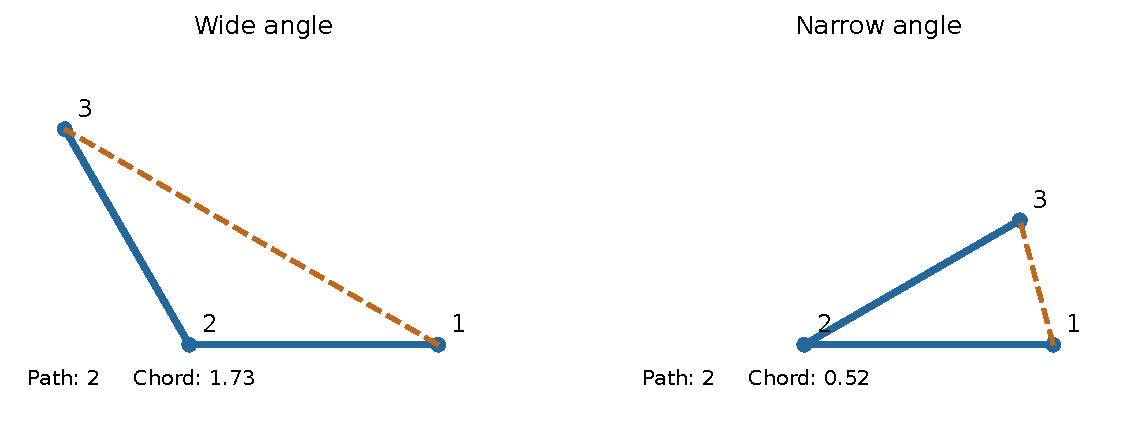
\includegraphics[width=.9\linewidth]{figures/focused/paths.pdf}
\caption{Two drawings of the same three-vertex unit path. Blue segments retain
length one, and the route from 1 through 2 to 3 retains length two. The orange
endpoint chord changes with the angle. Both drawings have zero edge and
fixed-path stress. All spatial units are equal.}\label{fig:paths}
\end{figure}

\subsection{Profiled scale and contraction}
Fitting a common target scale allows the input lengths to match the overall
size of the drawing. The effect on optimization becomes visible by expanding
the edge loss. The weighted squared sizes of the embedded and input edges are
$A=\sum_e\kappa_ed_e^2$ and $B=\sum_e\kappa_e\ell_e^2$; their weighted
cross-product is $C=\sum_e\kappa_ed_e\ell_e$. If $B>0$, the best target scale
is $a(Z)=C/B$. Substitution into \eqref{eq:edge} gives the profiled loss
\begin{equation}
 \E(Z)=\min_a E(Z,a)=\tfrac12(A-C^2/B).
 \label{eq:profile}
\end{equation}
\begin{proposition}[Homogeneity of the profiled loss]\label{prop:scale}
Hold the stiffnesses fixed and assume $B>0$.
For $c>0$, $a(cZ)=ca(Z)$ and $\E(cZ)=c^2\E(Z)$.
If $A>0$, the normalized quantity $Q=2\E/A=1-C^2/(AB)$ is invariant under
uniform coordinate scaling.
\end{proposition}
\begin{proof}
Scaling coordinates by $c$ multiplies $A$ by $c^2$ and $C$ by $c$, leaving
$B$ unchanged. Substitute these relations into \eqref{eq:profile}.
\end{proof}
A configuration with positive profiled loss has a strict descent direction
under uniform contraction. Thus no positive-loss local minimum exists in an
unconstrained configuration domain admitting such contractions. Wherever the
objective is differentiable, differentiating $\E(cZ)=c^2\E(Z)$ at $c=1$ gives
$\langle Z,\nabla\E(Z)\rangle=2\E(Z)$, with the Frobenius inner product.
A positive-loss stationary point is therefore impossible. If zero target
scale and collapsed coordinates are admitted, total collapse attains zero
loss. If scale must remain strictly positive, shrinking any configuration with
$C>0$ still drives the infimum to zero, even when no noncollapsed zero-residual
shape exists. These are properties of the unnormalized optimization problem
at fixed stiffnesses; they do not assert that every finite run collapses.
A small loss or gradient can reflect contraction without a change in relative
shape. Separately normalized diagnostics remain meaningful.
The optimal coordinate-scale calculation below is the weighted least-squares
calculation underlying scale-normalized graph stress
\citep[Section 3.2]{ahmed2026}; the additional issue here is profiling the
target scale while minimizing the unnormalized objective over coordinates.

For comparison, optimize the coordinate scale of a fixed shape against fixed
edge targets. If $A>0$ and $C>0$, $\min_{c>0}E(cZ,1)=B Q/2$, attained at
$c=C/A$. Thus a properly normalized shape loss and fixed-target fitting with
optimal overall size have related shape objectives. The raw profiled loss
\eqref{eq:profile} lacks this normalization. The present experiments use
fixed-target controls without introducing a new optimizer for $Q$.

\section{Expanding surfaces and their metric limits}
An elongated drawing can arise from the input distance geometry as well as
from the fitting criterion. The paraboloid and saddle separate these effects
because their smooth geodesic distances have explicit limits as the domain
radius grows. On both surfaces, horizontal dimensions grow as $r$ and heights
as $r^2$. Dividing intrinsic distances by $r^2$ reveals which separations
persist at the height scale.

\subsection{Paraboloid: a normalized line limit}
On the paraboloid $z=x^2+y^2$, height depends only on distance from the
vertical axis. To follow the same base locations as the domain expands,
fix points $u_i\in\R^2$ in the unit disk. Their squared radii
$q_i=\norm{u_i}^2$ determine the surface points
$P_i(r)=(ru_i,r^2q_i)$. The intrinsic geodesic distance between two such
points, restricted to the surface above the radius-$r$ disk, is $g_{ij}(r)$.
At the height scale, the distance is determined by vertical separation:
\begin{proposition}\label{prop:paraboloid}
For every pair and $r>0$,
\[
 r^2|q_i-q_j|\le g_{ij}(r)\le r^2|q_i-q_j|+(1+\pi)r.
\]
\end{proposition}
\begin{proof}
Every surface path has length at least its absolute vertical displacement.
For an upper bound, move radially from the outer endpoint to the inner radius,
then along the shorter circular arc. Since
$\sqrt{1+4\rho^2}\le1+2\rho$, the radial part is at most the height difference
plus $r$, and the arc is at most $\pi r$. This path stays in the disk.
\end{proof}
The normalized distances converge uniformly to $|q_i-q_j|$. Angular separation
vanishes at this scale; this does not mean its unscaled distance vanishes.

\begin{theorem}\label{thm:paraboloid}
Fix a finite sample with at least two distinct $q_i$ and a dimension $p\ge1$.
Every global raw-stress minimizer for $g(r)$, after division of coordinates
by $r^2$, has a centered Gram matrix converging to $(Jq)(Jq)^T$. The same
holds for classical MDS and for approximate raw-stress minimizers with
excess stress $o(r^4)$.
\end{theorem}
\begin{proof}
Writing $Z=r^2V$ divides the stress by $r^4$ and the targets by $r^2$.
The candidate $V_i=(q_i,0,\ldots,0)$ has normalized stress at most
$\binom n2(1+\pi)^2/r^2$. Minimizers, including the stated approximate ones,
therefore have residuals tending to zero. Their pair distances converge to
$|q_i-q_j|$, and double-centering their squared distances gives the Gram limit.
For classical MDS, $B(r)/r^4$ converges directly to the same rank-one matrix;
its unique positive eigenvalue is separated from zero.
\end{proof}
This is a fixed-sample result. It does not establish that the fitted optimizer
outputs attain its approximation requirement. For coupled samples whose
$q_i(r)$ converge, the same proof uses the moving line candidate and requires
at least two distinct limiting heights.

\subsection{Saddle: a tree metric with three-dimensional classical span}
On the saddle, equal height does not always allow a connection that stays at
that height. Positive levels have two components, as do negative levels.
This separation determines the limiting distances. Fix $(a_i,b_i)$ in the
unit disk and write the corresponding points on $z=x^2-y^2$ as
$P_i(r)=(ra_i,rb_i,r^2h_i)$, where $h_i=a_i^2-b_i^2$ and $t_i=|h_i|$.
Positive heights have separate $+x$ and $-x$
branches; negative heights have separate $+y$ and $-y$ branches. Zero heights
map to a common root. Define the four-branch tree distance
\begin{equation}
 T_{ij}=\begin{cases}|t_i-t_j|,&i,j\text{ on the same branch},\\
 t_i+t_j,&i,j\text{ on different branches}.
 \end{cases}\label{eq:tree}
\end{equation}
\begin{proposition}\label{prop:saddle}
The intrinsic saddle distances on the disk-restricted patch satisfy
$r^2T_{ij}\le g_{ij}(r)\le r^2T_{ij}+4r$.
\end{proposition}
\begin{proof}
Length dominates total vertical variation. Different signs of height require
crossing zero. Opposite positive branches require $x$ to cross zero, where
height is nonpositive; opposite negative branches similarly require $y$ to
cross zero. These facts give the lower bound.

For the upper bound, follow each constant-height hyperbola to its corresponding
coordinate semiaxis. On a positive branch, $|dx/dy|\le1$ and
$|y|\le r/\sqrt2$, so each connector has length at most $r$; negative branches
exchange $x$ and $y$. Connect the semiaxis points monotonically on one branch
or through the origin for different branches. The inequality used in
Proposition~\ref{prop:paraboloid} bounds this segment by the required vertical
variation plus $2r$. All segments remain inside the disk. Zero-height points
follow a straight ruling to the origin.
\end{proof}
Thus $g(r)/r^2\to T$ uniformly. The limit is intrinsically a one-dimensional
tree. Its classical Euclidean approximation need not be one-dimensional.

To determine the Euclidean span selected by classical MDS, encode each
point by its distance from the root in its branch coordinate. In the next
statement, $e_b$ denotes the $b$th standard basis vector of $\R^4$.
\begin{theorem}\label{thm:saddle}
Let $F$ be the $n\times4$ matrix with row $t_i e_{a(i)}^T$ for a nonroot point,
where $a(i)$ is its branch label, and zero row for a root point.
If $JF$ has rank four, the double-centered Gram matrix
$-\tfrac12JT^{\circ2}J$ has exactly three positive eigenvalues and one negative eigenvalue.
Classical three-dimensional MDS of the expanding saddle therefore retains
three nonzero limiting singular values after coordinate division by $r^2$.
\end{theorem}
\begin{proof}
Since $t=F\one$, expansion of \eqref{eq:tree} and double-centering give
\begin{equation}
 B_T=-\tfrac12JT^{\circ2}J
     =JF(2I_4-\one\one^T)F^TJ.\label{eq:tree-gram}
\end{equation}
The middle matrix has eigenvalues $2,2,2,-2$. The full column rank of $JF$
transfers these nonzero inertia counts to $B_T$. Proposition~\ref{prop:saddle}
implies $B(r)/r^4\to B_T$, so the three positive classical directions persist.
\end{proof}
A sufficient rank condition is one nonroot observation per branch and two
distinct positive lengths on at least one branch. A root plus one nonroot
point per branch also suffices. Missing branches or degenerate samples need
separate analysis. The theorem applies to classical scaling; it does not
exclude every planar minimizer of raw stress on the tree metric.
Non-Euclidean Gram spectra for tree metrics are already illustrated by the
three-leaf-star example of \citet[Example~2.6]{lim2024}. Here the surface
distance bound identifies the tree arising from the expanding saddle, and
the rank condition identifies when its classical approximation retains three
positive directions.

A simple example makes the spatial dimension concrete. Four branch tips at
unit distance from the root have pairwise distances two. If only these tips
are observed, their centered matrix is $2J$, and classical MDS represents them
exactly as a regular tetrahedron. A planar cross has the right tree routes
but not these Euclidean endpoint distances. This tip-only sample has rank
three in $JF$ and illustrates why the rank-four condition above is sufficient,
not necessary, for a three-dimensional classical span.

Gaussian curvature alone does not resolve this comparison. On these two
surfaces, curvature is respectively $4/(1+4\rho^2)^2$ and
$-4/(1+4\rho^2)^2$. Their magnitudes decay identically with radius, yet their
normalized distance limits differ because of the connectivity of height
levels. Figure~\ref{fig:ratios} shows the corresponding finite-sample behavior.

This explanation can be stated using Reeb graphs. On the unit disk, collapse
each connected level component of $q(u)=\norm{u}^2$ or $h(a,b)=a^2-b^2$ to a
point. Give a path in the quotient its total variation in function value,
as in the metric Reeb construction \citep[Definitions 2.1 and 3.1]{memoli2023reeb}.
Both height functions are 1-Lipschitz for their normalized surface distances.
For $q$, the quotient is $[0,1]$ with ordinary distance. For $h$, positive and
negative levels each have two components, joined at the connected zero level;
the quotient is the four-branch tree in \eqref{eq:tree}. Propositions
\ref{prop:paraboloid} and \ref{prop:saddle} supply explicit uniform distance
errors for these particular quotients. The identification uses this established
construction, without requiring a general collapse theorem.

\begin{figure}[tb]
\centering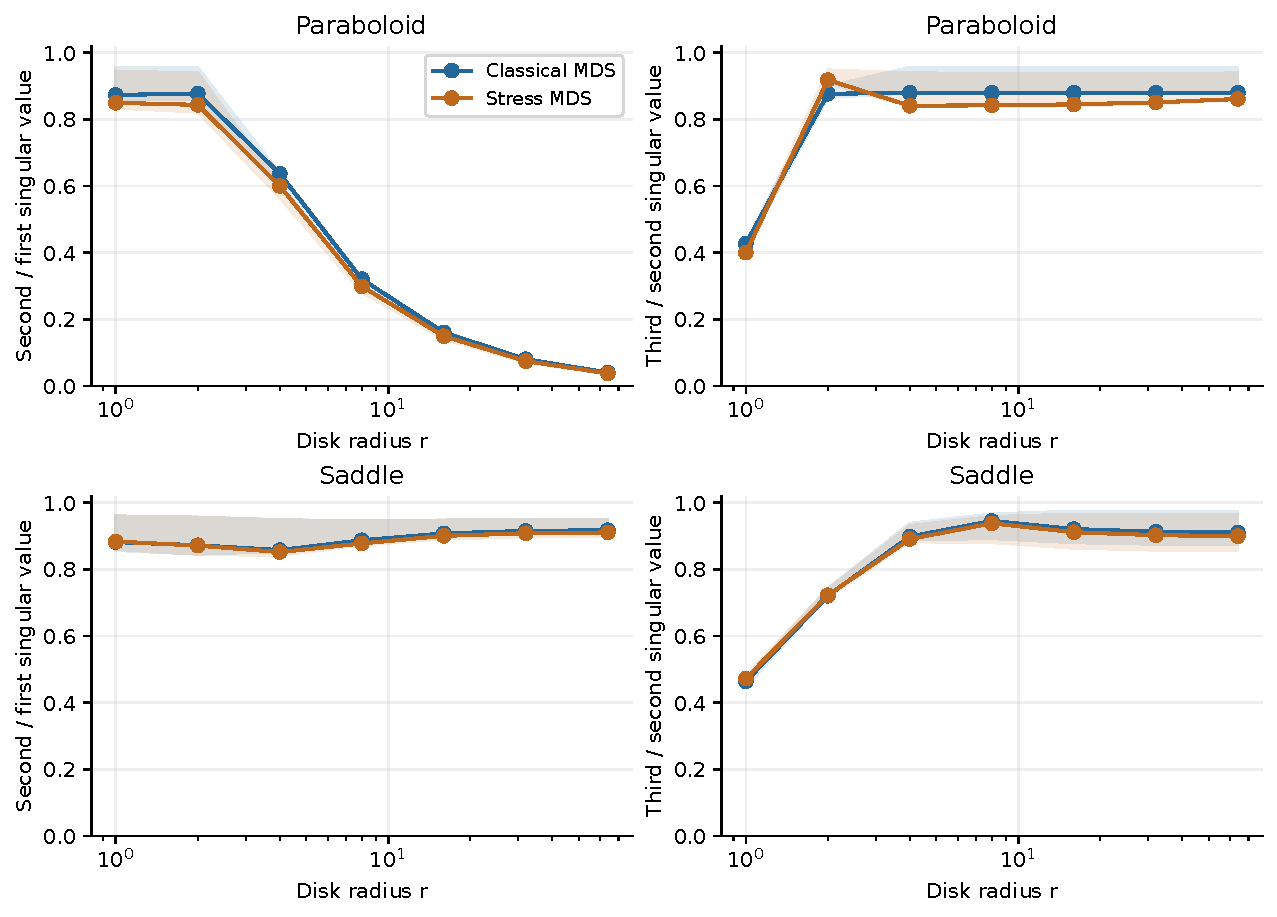
\includegraphics[width=.9\linewidth]{figures/focused/shape-ratios.pdf}
\caption{The expanding paraboloid becomes elongated, while the saddle retains
three comparable embedding directions. Shape ratios are shown for complete
geodesic graphs ($n=240$, $k=239$), under base-disk sampling. Curves show medians and bands the observed ranges across
three samples. Both ratios are needed: two small transverse directions can
remain comparable while the configuration approaches a line. These are
classical and finite-budget stress-MDS fits to strict graph distances; numerical
smooth-geodesic targets and their strict distances can differ slightly.
The classical and global raw-stress statements have the separate assumptions
in Theorems~\ref{thm:paraboloid} and \ref{thm:saddle}.}\label{fig:ratios}
\end{figure}

\section{Controlled experiments}
The surface limits describe intrinsic distances and idealized MDS behavior.
The experiments examine what happens when a sampled neighborhood graph and
a finite optimization budget intervene. One study isolates the choice of MDS
initializer on a bounded saddle. The other varies radius, graph construction
and scale on both surfaces. Their designs differ, so each comparison retains
its own samples, targets and scale policy.

\subsection{Bounded-saddle initializer comparison}
The first study uses five independent area-uniform samples of $n=1{,}000$
points on $z=0.8(x^2-y^2)$ over $[-1,1]^2$. Symmetric-union kNN graphs use
ambient chord lengths both for neighbor selection and as edge targets.
The selected neighborhood sizes are 71, 70, 67, 72 and 73, based on comparison
with numerical surface-geodesic references. This calibration minimizes
unscaled graph-to-reference relative RMSE over $k=3,\ldots,80$, using 119,744
unordered pairs obtained from 128 reference sources and all targets. It uses
the known surface and is not a neighborhood-selection rule for unknown
biological geometry. Each sample additionally uses
$k=32$, $k=80$, and the selected $k\pm5$, giving 25 graphs. These graphs are
connected without added bridges.

Classical and raw-stress MDS use strict graph shortest-path matrices and
three output dimensions. Stress MDS selects the least achieved stress from
six starts: one classical and five Gaussian, with 1,000 iterations per start.
Both branches then receive the same five-stage edge-KK schedule, interpolating
from density stiffness to uniform stiffness with 200 steps per stage. This
historical comparison uses the profiled target scale. The Gaussian draws are
paired across $k$ within each sample. Additional iterations are controls and
do not replace the primary fits.

\subsection{Radius, graph, and scale comparison}
The second study samples $z=x^2+y^2$ and $z=x^2-y^2$ above disks with
$r\in\{1,2,4,8,16,32,64\}$. For each surface, both uniform base-disk and uniform
surface-area sampling are considered, with three independent $n=240$ samples
and coupled quantiles/angles across radii. No uniform probability distribution
on the entire infinite-area surface is assumed.

The neighborhood grid is $k\in\{4,8,16,32,64,128,239\}$. Separate graph regimes
use either numerical smooth geodesics or ambient chords for both ranking and
edge targets. Graphs are symmetrized by union; minimum-spanning-tree edges
repair disconnected cases and are recorded. Classical and stress MDS use each
graph's strict distances. Stress MDS uses one classical and two Gaussian starts,
each limited to 1,000 iterations. In the geodesic regime, a full-surface-distance
classical initializer held fixed across $k$ is an additional control.

Every initializer receives both density continuation and an equal-budget
uniform-only refinement, under both profiled and fixed target scales.
The primary schedule has the same five mixing values and 1,000 total steps
as the first study. Numerical inputs are scaled by the RMS smooth distance
within each case and outputs are restored to physical units. The fixed target
scale is one in these normalized fitting units.

A nested $n=480$ sample at $r=64$ retains the original 240 points of replicate
one and uses $k\in\{8,16,64,128,479\}$. Perturbation, additional-iteration,
random-start and original-coordinate controls use 32 selected high-radius
settings. Shared original/random controls appear in more than one branch
comparison and do not supply independent replications.

\subsection{Diagnostics and numerical validation}
Separating relative geometry from overall size requires an explicit scale
convention for each diagnostic. For a positive target vector $t$ and an
achieved length vector $y$, the least-squares calibration of the targets is
$b=\langle y,t\rangle/\norm{t}^2$. Edge and retained-path relative errors are
$\norm{y-bt}/\norm{bt}$, each with its own diagnostic calibration. Chord
Stress-1 uses $\norm{y-bt}/\norm{y}$. These scale conventions are explicit
because normalizations called stress are not interchangeable \citep{mair2022}.
Graph-to-surface distance error uses common physical units. Embedded
path-to-surface error uses the calibration estimated from graph edges, so it
does not fit a new scale against the surface reference.

Recovery of the generating configuration requires a separate comparison of
coordinates. Coordinate error is a normalized Procrustes residual after translation,
orthogonal transformation and one uniform scaling, with vertex correspondence
retained. It is not the percentage of misclassified observations. Singular
values $s_1\ge s_2\ge s_3$ distinguish elongation ($s_2/s_1$ small) from
planarity relative to the second direction ($s_3/s_2$ small). Neither is a
certificate of topology or surface recovery.
To assess horizontal and vertical recovery separately, we also split the
residual from this same global similarity alignment into its $(x,y)$ and $z$
components, dividing each norm by the corresponding centered truth norm.
No additional component-specific rotation or scale is fitted. Component errors can exceed one. These
errors reveal distortions that the global norm can conceal when height dominates.

The radius study contains \numRadiusGraphs{} primary graphs, \numRadiusCandidates{} scored primary
configurations and \numRadiusStarts{} MDS starts; \numRepairedGraphs{} graphs require connectivity repair.
All \numInputMatrices{} numerical input matrices pass symmetry, chord lower bounds,
constructed surface-path upper bounds and exhaustive vertex-triple checks
within $10^{-7}$ times RMS distance. Independent high-radius numerical
validation covers \numValidationPairs{} actual pairs in 16 cases, with maximum sampled relative
discrepancy $\numGeodesicDiscrepancy$. This is not a certified all-pairs accuracy bound.
Independent reconstruction from \numValidatedCoordinates{} primary and control
coordinate arrays checks singular-value quantities, edge calibration and error,
raw chord stress, chord Stress-1, coordinate error, and graph-to-surface error.
These diagnostics agree to $\numCoordinateDiscrepancy$ after dimensional scaling;
this full validator does not reconstruct retained-path scores.
Path validation is separate: fitting-time checks compare with the package
scorer and explicitly sum 31 routes per configuration. An additional ordinary-R
calculation sums all 28,680 retained routes in each of 24 configurations at
$n=240$, $r=64$, $k=32$, spanning both surfaces, three base-disk replicates,
both graph regimes, and stress fits before and after fixed-scale density
continuation. Retained-path and path-to-surface errors agree with the frozen
scores to $\numRetainedRouteDiscrepancy$ in absolute error units.
The retained near-tie routes and strict matrices are recorded separately.

\section{Results}
\subsection{Path improvement and geometric agreement}
In the bounded-saddle comparison, refinement improves path agreement while
worsening normalized chord agreement. Edge-KK decreases
retained-path error in all \numBoundedGraphs{} bounded-saddle settings under
both initializers and increases chord Stress-1 in all corresponding comparisons.
At the selected graphs, median path error decreases from \numClassicalBefore\% to \numClassicalAfter\%
for classical initialization and from \numStressBefore\% to \numStressAfter\% for stress
initialization (Table~\ref{tab:initializers}, Figure~\ref{fig:initializers}).
Stress initialization gives the lower final path error in \numStressWins{} of \numBoundedGraphs{} graphs,
with two reversals retained in the comparisons.

Coordinate agreement does not follow the same pattern. The median coordinate
error increases under classical initialization, while decreasing slightly
under stress initialization. Across selected graphs, stress-initialized
refinement gives coordinate errors ranging from \numCoordLow\% to \numCoordHigh\% despite
small final path errors. All recorded edge-KK stages reach their iteration
limits. These are achieved finite-budget outcomes, not established minima.

\begin{table}[tb]\centering\small
\caption{Path agreement improves after edge-KK while chord agreement worsens:
bounded-saddle medians over five selected graphs. Retained-path and edge
columns use separately calibrated relative errors; chord is profiled Stress-1;
coordinate error uses similarity alignment. Edge-KK uses the historical
profiled scale.}\label{tab:initializers}
\begin{tabular}{lrrrr}
\toprule
Method & Retained path (\%) & Edge (\%) & Chord (\%) & Coordinate (\%)\\
\midrule
Classical MDS & 3.451 & 7.133 & 3.459 & 29.19\\
Stress MDS & 2.264 & 5.081 & 2.803 & 23.20\\
Classical MDS + edge-KK & 0.245 & 0.382 & 4.715 & 30.67\\
Stress MDS + edge-KK & 0.164 & 0.227 & 5.213 & 22.32\\
\bottomrule
\end{tabular}

\end{table}
\begin{figure}[tb]\centering
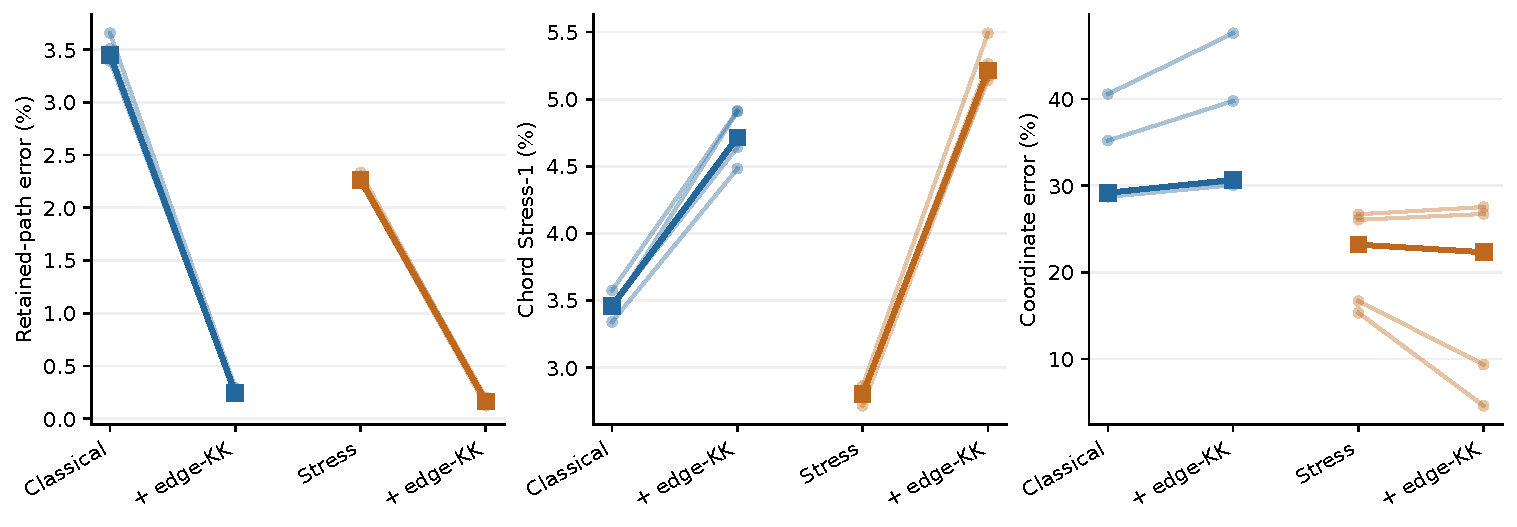
\includegraphics[width=\linewidth]{figures/focused/initializer-comparison.pdf}
\caption{Path, chord and coordinate errors respond differently to edge-KK.
Paired bounded-saddle comparisons use the selected graphs. Thin lines
join the same sample before and after edge-KK; squares show medians over five
samples. Blue denotes classical initialization and orange stress initialization.
Vertical units and ranges differ across the three diagnostics.}\label{fig:initializers}
\end{figure}

\subsection{Graph fidelity and coordinate recovery separate on the saddle}
The large-radius saddle makes the difference between intrinsic-distance
agreement and coordinate recovery particularly clear. At $r=64$, $k=32$,
the fixed-scale stress-initialized geodesic saddle fits
have median path-to-surface error \numGeodesicSaddlePath\% and coordinate error \numGeodesicSaddleCoord\%.
Ambient-graph fits give \numAmbientSaddleCoord\% coordinate error but \numAmbientSaddlePath\% path-to-surface
error (Table~\ref{tab:radius}). The geodesic fits preserve intrinsic path
measurements much better; the ambient fits have much smaller global coordinate
residuals. These outcomes answer different geometric questions, and the global
residual alone does not establish detailed surface recovery.
Figure~\ref{fig:spatial} shows the corresponding configurations for the first
sample, together with the smaller-radius comparison. The original surface
extends over the entire disk at both radii. Its horizontal extent grows as
$r$ and its vertical extent as $r^2$, so equal-axis views become narrow at
large $r$. That ambient aspect ratio does not make the intrinsic saddle
distance metric a line metric.

Height dominates the global coordinate norm on both surfaces at this radius.
For the ambient saddle, the median horizontal error after the same alignment
is \numAmbientSaddleHorizontal\%, despite a global error of
\numAmbientSaddleCoord\% and a vertical error of \numAmbientSaddleVertical\%
(Table~\ref{tab:components}). Simply setting the original horizontal coordinates
to zero gives a height-only saddle configuration with median global residual
\numAmbientSaddleHeightOnly\%, even before optimizing its alignment. The ambient
fits improve on that baseline, but their small global residual does not certify
recovery of the sampled disk. The paraboloid fits are strongly elongated under
both graph regimes: their median horizontal errors are
\numAmbientParaboloidHorizontal\% for ambient graphs and
\numGeodesicParaboloidHorizontal\% for geodesic graphs. Component errors, as well
as the shape ratios, are needed to assess transverse geometry.

\begin{table}[tb]\centering\small
\caption{Graph construction separates path agreement from coordinate recovery
on the saddle. Radius-study medians over three base-disk samples at $r=64$, $k=32$,
using stress MDS followed by fixed-scale density continuation. Retained-path/surface error uses edge
calibration; coordinate error uses similarity alignment.}\label{tab:radius}
\begin{tabular}{llrrrr}
\toprule
Surface & Graph & $s_2/s_1$ & $s_3/s_2$ & Coordinate (\%) & \shortstack{Retained path/\\surface (\%)}\\
\midrule
Paraboloid & geodesic & 0.038 & 0.846 & 1.46 & 0.34\\
Paraboloid & ambient & 0.028 & 0.915 & 0.88 & 0.38\\
Saddle & geodesic & 0.901 & 0.896 & 80.38 & 0.36\\
Saddle & ambient & 0.019 & 0.917 & 0.90 & 37.00\\
\bottomrule
\end{tabular}

\end{table}
\begin{table}[tb]\centering\small
\caption{Small global coordinate residuals can conceal horizontal distortion.
Medians over the same three base-disk samples and fits as Table~\ref{tab:radius}.
Horizontal and vertical errors use components of one globally aligned residual,
normalized by their respective centered truth norms. No separate alignment is
performed for either component. Component errors can exceed 100\% when the
residual exceeds the corresponding truth norm.}\label{tab:components}
\begin{tabular}{llrrr}
\toprule
Surface & Graph & Global (\%) & Horizontal (\%) & Vertical (\%)\\
\midrule
Paraboloid & ambient & 0.88 & 23.66 & 0.046\\
Paraboloid & geodesic & 1.46 & 38.58 & 0.197\\
Saddle & ambient & 0.90 & 35.24 & 0.025\\
Saddle & geodesic & 80.38 & 1751.52 & 65.930\\
\bottomrule
\end{tabular}

\end{table}
\begin{figure}[!t]\centering
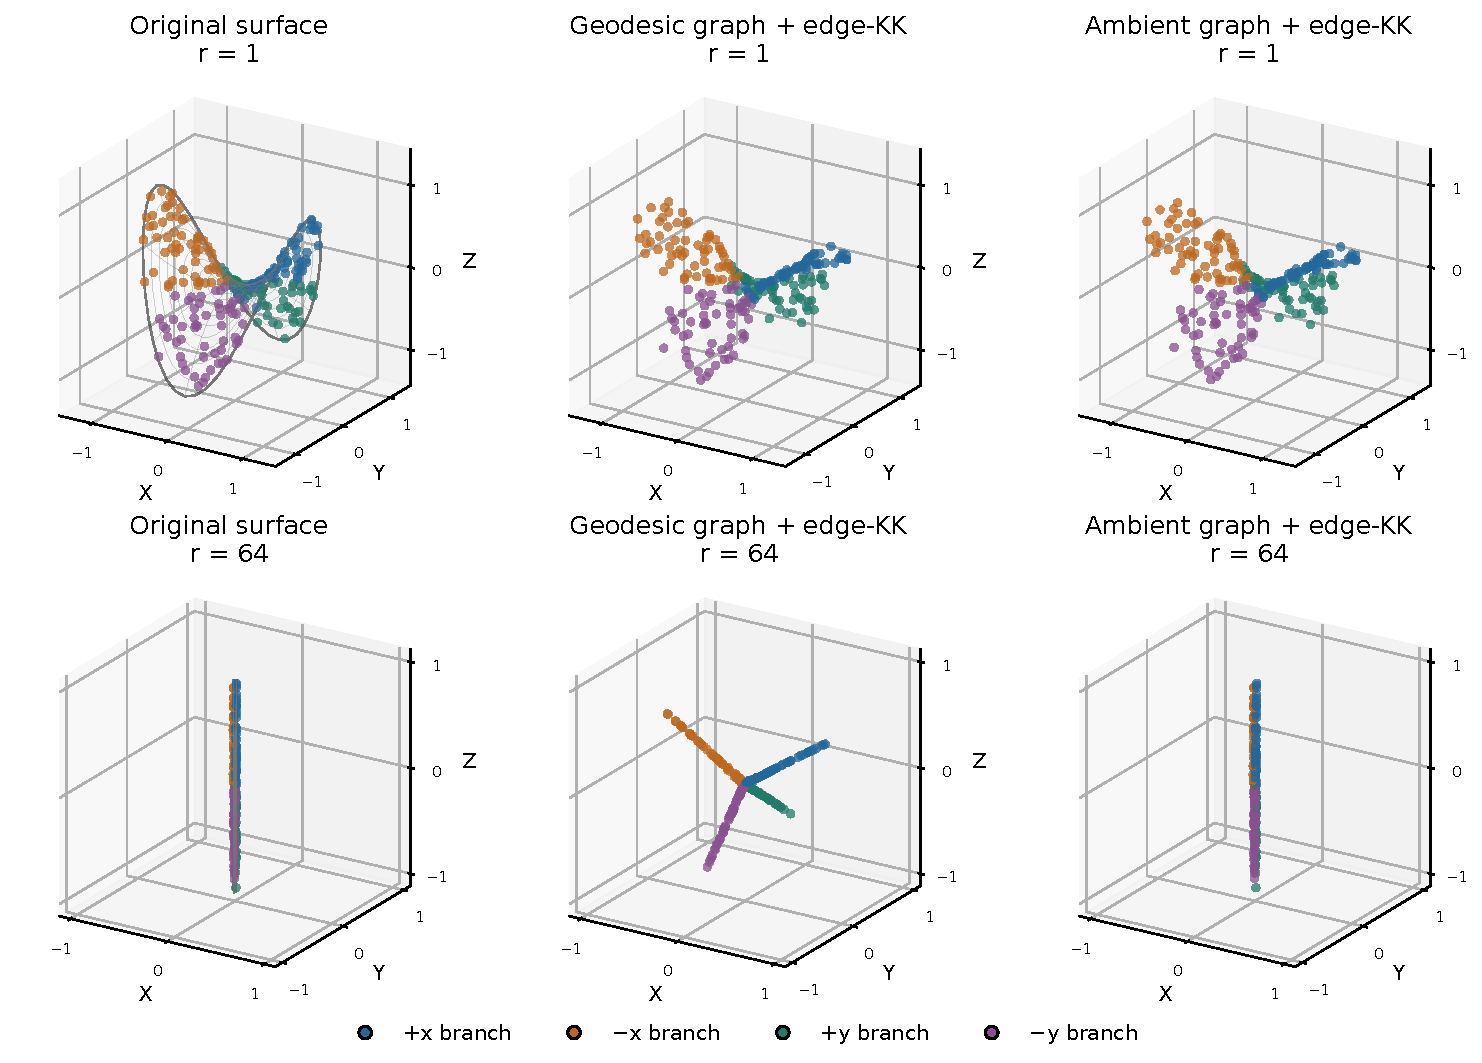
\includegraphics[width=.9\linewidth]{figures/focused/saddle-spatial.pdf}
\caption{Geodesic and ambient graphs produce different saddle configurations
as the domain expands. Shown is the first base-disk sample, $n=240$, $k=32$.
The fitted columns use stress MDS followed by fixed-scale density continuation.
Colors identify the four original height-level branches. The original-surface
wireframe includes the full disk boundary. All coordinates are centered and
divided uniformly by $r^2$; fitted coordinates are also divided by their edge
calibration factor and orthogonally aligned to the original observations.
Each row uses common limits, equal spatial axes and an orthographic view.
At $r=64$ the original disk's horizontal radius in these units is $1/64$,
which explains its narrow appearance. No coordinate direction is enlarged
independently.}\label{fig:spatial}
\end{figure}

\subsection{Neighborhood and initialization sensitivity}
Changing the neighborhood size changes both the graph approximation and the
constraints imposed during refinement. Graph-to-surface and embedded-path-to-surface errors vary with $k$
(Figure~\ref{fig:graph}). A small graph-to-layout error cannot repair a
substantial graph-to-surface error. Even when the full-geodesic classical
initializer is held fixed across $k$, final path-to-surface error changes
with the refinement graph in all \numFullInitializerCases{} corresponding $n=240$ cases.
Across the seven tested $k$ values, the within-case range of that error has
median \numNeighborhoodSpreadMedian{} percentage points, with ranges from
\numNeighborhoodSpreadMin{} to \numNeighborhoodSpreadMax{} percentage points
across cases. These are changes in error magnitude, not independent replications
or estimates of uncertainty in a preferred $k$.

The nested sample-size check distinguishes fixed $k$ from fixed $k/n$.
For example, under geodesic construction and fixed-scale refinement on the
base-disk paraboloid, path-to-surface errors are \numNestedBase\% for $(n,k)=(240,8)$,
\numNestedSameK\% for $(480,8)$, and \numNestedSameFraction\% for $(480,16)$. This single nested
replication does not establish a general sample-size scaling law.

Tiny perturbations around stress-MDS starts change the final $s_3/s_2$
ratios by at most \numStressPerturbation{} across the tested controls; the
corresponding maximum around classical starts is \numClassicalPerturbation{}.
Independently drawn starts can give much larger changes, up to approximately
\numStressRandomFixed{} under fixed scale. Local stability around an initializer
therefore does not imply insensitivity to its selection. Of the
\numRadiusStarts{} primary radius-study MDS starts, \numCappedStarts{} reach their
iteration caps; small stress changes are not a global-optimality certificate.
\subsection{Contraction and fixed-scale controls}
Allowing the target scale to vary can produce substantial contraction of the
drawing. Across all primary refinements, including both sample sizes, all initializers
and both stiffness schedules, the profiled-scale runs attain edge calibration
factors as small as $\numProfiledMinimum$. Among \numProfiledCount{} profiled
refinements, \numProfiledBelowHalf{} have calibration below $0.5$,
\numProfiledBelowTenth{} below $0.1$, and \numProfiledBelowThousandth{} below
$0.001$; the median is \numProfiledMedian{}. These nested counts describe
correlated configurations in the declared grid. The fixed-scale controls range from
\numFixedMinimum{} to \numFixedMaximum{}.
Contraction occurs at intermediate radii as well as large ones, so it is not
an asymptotic property of the generating surface (Figure~\ref{fig:scale}).

Across the \numPrimaryGraphs{} primary $n=240$ graphs, profiled-scale refinement improves
path error in \numProfiledImproved{} stress-initialized comparisons, worsens it in \numProfiledWorsened{}, and
leaves \numProfiledTied{} ties. Fixed-scale refinement improves \numFixedImproved{}, worsens \numFixedWorsened{}, and leaves
\numFixedTied{} ties. Ties mean absolute changes no larger than $10^{-8}$ in relative-error
units. These counts describe the declared graph grid, not independent trials
or probabilities for future data. Neither policy improves path error in every
case. Fixed scale removes the contraction mechanism of Proposition~\ref{prop:scale};
nonconvexity and geometric ambiguity remain.

\subsection{Density continuation and uniform stiffness}
Density continuation is the primary protocol, but the paired uniform-only
controls do not show a consistent advantage for it. Holding the initializer,
graph, scale policy and total step budget fixed, continuation yields lower
retained-path error in 389 of 1,176 fixed-scale stress comparisons, higher error
in 541, and ties in 246 (Table~\ref{tab:continuation}). The central half of paired
changes is small, while the extremes are larger, particularly for coordinate
error. Profiled-scale comparisons also favor neither schedule uniformly.
The results establish schedule sensitivity at the achieved finite budgets;
they do not demonstrate that continuation improves on uniform stiffness.

\begin{table}[htbp]\centering\small
\caption{Density continuation minus uniform-only error for paired stress-initialized
radius-study fits, with 1,176 primary $n=240$ graphs per scale policy. Negative
changes favor continuation. Counts use an absolute tie tolerance of $10^{-8}$
in relative-error units; intervals and medians are in percentage points (pp).
The pairs share graphs and samples and are not independent trials.}\label{tab:continuation}
\begin{tabular}{llrrr}
\toprule
Scale & Error & \shortstack{Lower/higher/\\tied} & \shortstack{Median [quartiles]\\(pp)} & \shortstack{Minimum, maximum\\(pp)}\\
\midrule
Profiled & Retained path & 411/627/138 & 0.0000 [-0.0007, 0.0061] & -0.190, 0.349\\
Profiled & Coordinate & 432/614/130 & 0.0001 [-0.0030, 0.0271] & -1.832, 9.940\\
Fixed & Retained path & 389/541/246 & 0.0000 [-0.0003, 0.0072] & -0.357, 0.470\\
Fixed & Coordinate & 397/567/212 & 0.0000 [-0.0044, 0.0412] & -1.952, 9.380\\
\bottomrule
\end{tabular}

\end{table}

\begin{figure}[p]\centering\small
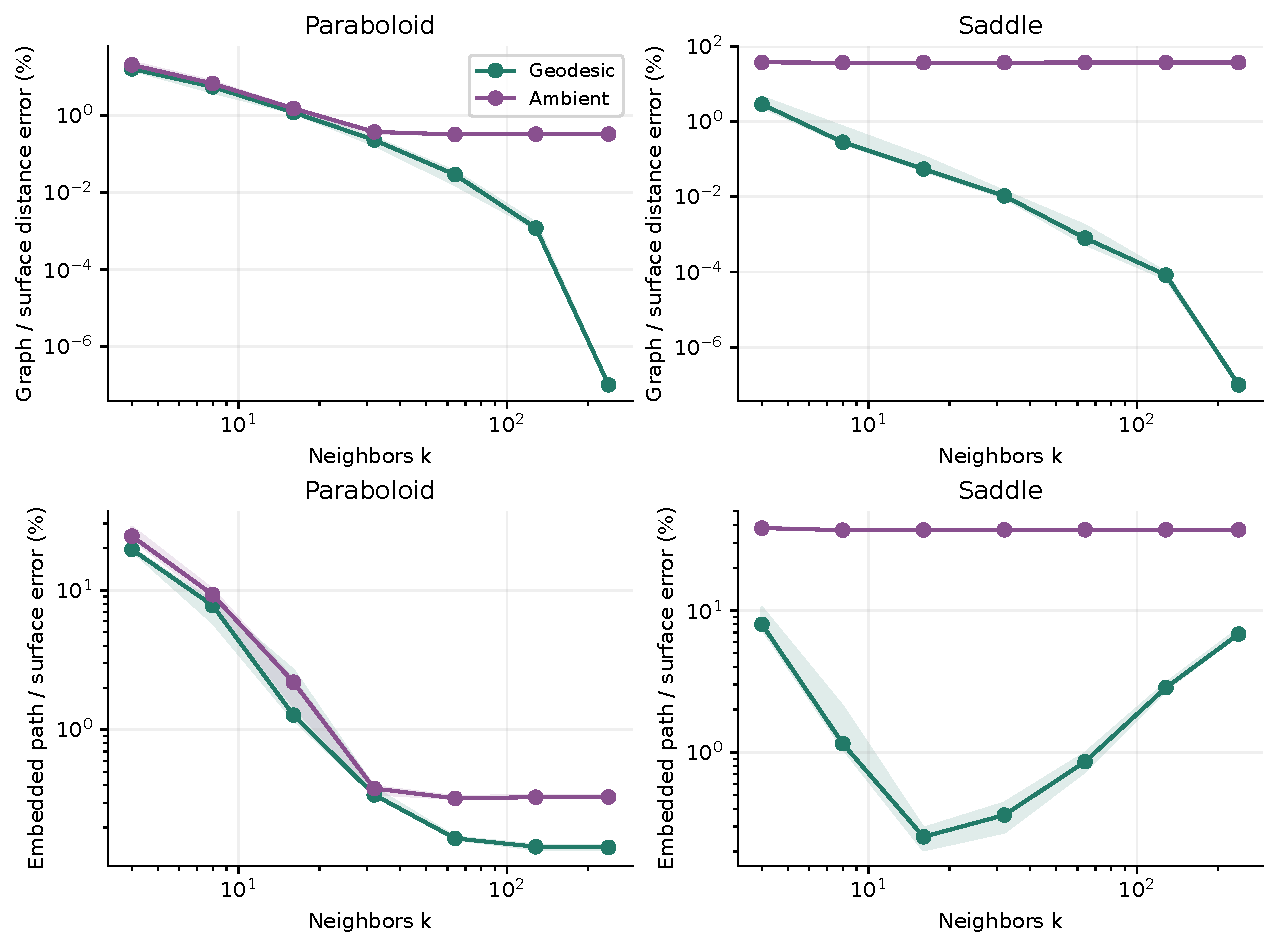
\includegraphics[width=.82\linewidth]{figures/focused/graph-sensitivity.pdf}
\caption{Neighborhood size affects graph-to-surface and embedded-path-to-surface
agreement at $r=64$ under base-disk sampling. Curves
are medians and bands observed ranges over three samples. The upper row
compares strict graph distances with numerical smooth geodesics. The lower
row compares edge-calibrated retained paths after fixed-scale, stress-initialized
edge-KK with the same reference. Panels use separate logarithmic ranges;
values below $10^{-7}$\% are drawn at that display floor.}\label{fig:graph}
\par\vspace{1ex}
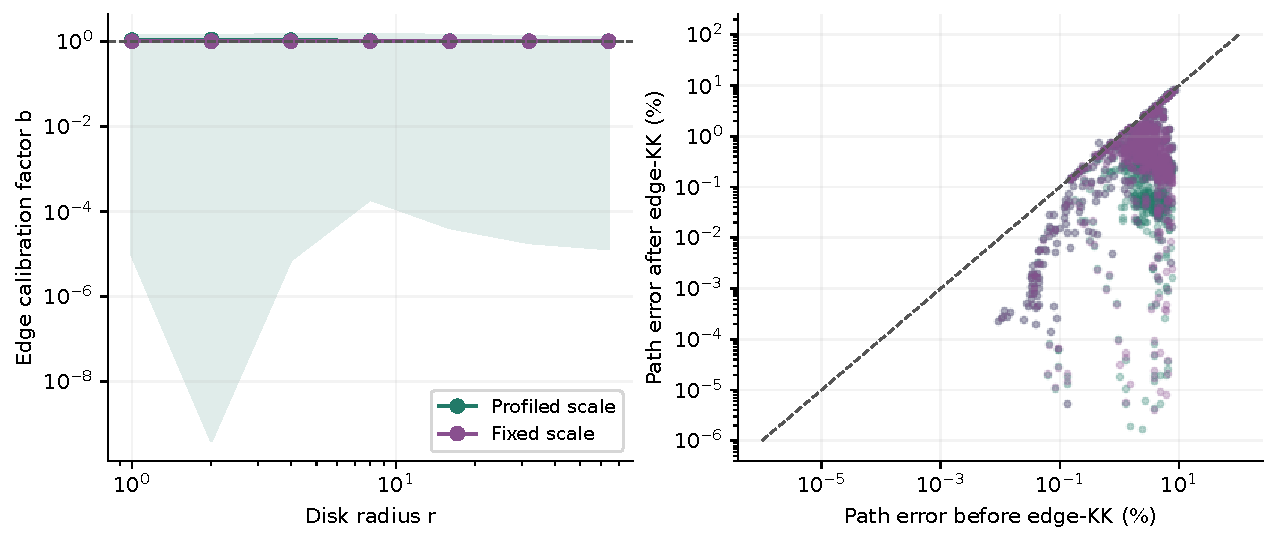
\includegraphics[width=.88\linewidth]{figures/focused/scale.pdf}
\caption{Scale and normalized path fidelity are separate diagnostics.
Left: median and full observed range of the edge calibration factor for
stress-initialized density continuation across all primary $n=240$ settings at each radius. Right: paired path errors before
and after stress-initialized edge-KK; points below the diagonal improve.
Pairs with either error at most $10^{-8}$ are omitted from this logarithmic
scatter only; all comparisons enter the reported counts.}\label{fig:scale}
\end{figure}

\FloatBarrier
\section{Discussion}
An embedding is useful only in relation to the measurements it is intended
to support. In these experiments, accurate lengths along retained graph paths
can coexist with substantial coordinate error, while close coordinate
agreement can coexist with poor intrinsic-distance agreement. The distinction
begins at graph construction: a drawing that faithfully represents a chosen
graph still inherits that graph's approximation to the underlying geometry.
When the reference surface is unknown, graph-to-layout agreement can assess
the embedding step but cannot verify the scientific meaning of the graph.

The surface limits explain one source of this separation. At the height
scale, the paraboloid loses angular separation and approaches a line metric.
The saddle retains the separation of four height-level branches and
approaches a tree metric. Under the stated rank condition, classical MDS
represents the latter with three nonzero limiting directions. A
one-dimensional intrinsic structure therefore need not give a one-dimensional
Euclidean embedding. The raw-stress fits also retain broad three-dimensional
span in the tested saddle settings, although a universal raw-stress result
has not been established. Curvature decay or a quadratic fit to the displayed
coordinates alone cannot distinguish these distance geometries.

On flexible graphs, path fidelity leaves geometric freedom: edge lengths can
be preserved while angles change. This counterexample does not diagnose the
dense experimental graphs. In the ambient regime, the original coordinates
realize every target edge exactly. For the three highlighted ambient saddle
frameworks at $n=240$, $r=64$, $k=32$, the edge-length Jacobian at the original
coordinates has numerical rank $714=3n-6$. Its smallest nongauge singular
values range from $0.00490$ to $0.00613$, whereas the six rigid-motion values
are of order $10^{-15}$. This supports local infinitesimal rigidity at those
frameworks, not global rigidity or a quantitative stability theorem
\citep{gortler2010}. The experiments do not identify which combination of
finite-budget optimization, conditioning and alternative global realizations
accounts for each coordinate residual. A small average edge error also
supplies less control than the uniform bound in Proposition~\ref{prop:path}.
Initialization or regularization can select among configurations with similar
path errors; their influence is part of the interpretation. Likewise, a
decreasing objective must be read together with its scale convention. The
profiled edge loss can fall under contraction without a change in relative
shape. Fixed target scale removes this mechanism, but the observed path-error
increases show that it does not ensure improvement in every graph or eliminate
dependence on initialization.

For biological observations, these distinctions affect how a branch, gap or
sequence of nearby samples can be interpreted. Stability to plausible graph
and embedding choices can support an interpretation of the drawing, while
biological evidence must establish what those relationships mean. The
synthetic examples isolate geometric effects; they do not establish
biological trajectories or validate features of a particular microbiome
dataset.

The comparisons concern two quadratic surface families and finite
optimization budgets. In the primary radius study, domain size increases
with sample size held fixed, so the samples do not become increasingly dense
surface meshes. Surface-area and base-disk sampling also assign different
weights to the geometry. The bounded-saddle study differs from the radius
study in domain, sample size and scale policy, and their scores cannot be
pooled. Within these designs, the separate path, endpoint, scale and
coordinate diagnostics identify which aspects of an embedding improve and
which remain undetermined.

\clearpage
\appendix
\section{Computational details}\label{app:computation}
\subsection{Sampling and geodesic references}
Uniform sampling in the base disk and on the surface weights radial positions
differently. For both radius-study surfaces the area element in polar base coordinates is
$\rho\sqrt{1+4\rho^2}\,d\rho\,d\theta$. Thus surface-area sampling uses the
radial cumulative distribution
\[
 F_r(\rho)=\frac{(1+4\rho^2)^{3/2}-1}{(1+4r^2)^{3/2}-1},
 \qquad 0\le\rho\le r,
\]
with independent uniform angle; base-disk sampling uses $F_r(\rho)=\rho^2/r^2$.
The same uniform draws are transformed at each radius. The primary NumPy
generator seeds are $20260904+j$ for replicate $j$. The nested additional
240 observations use seed 20261905. Corresponding surface/measure settings
share these draws, so settings are paired rather than independent samples.

Paraboloid distances use the radial first integral of the geodesic equations,
with separate turning and monotone radial paths and 62 bisection steps for
the angular boundary condition. Saddle distances use shooting for the
Cartesian geodesic equations in base coordinates scaled by $r$, with
continuation from smaller radii. The primary endpoint tolerance is
$2\times10^{-9}$ in these base units; the integration relative tolerance is
$2\times10^{-10}$. High-radius validation uses tighter shooting and independent
collocation/integration on the saddle, and refined radial solves with adaptive
quadrature on the paraboloid. The reported maximum concerns the selected
validation pairs, not an error guarantee for all pairs. The bounded-saddle
calibration uses a separate triangulated-surface reference, with mesh-refinement
and smooth-geodesic boundary-value checks recorded in its original protocol.

\subsection{Why complete-surface geodesics stay inside the disk}
The smooth solvers do not impose a reflecting or obstacle boundary at the disk
edge. This agrees with the stated surface-patch distance. To see this, write
$f(x,y)=x^2+\eta y^2$, $\eta\in\{-1,1\}$, and let $u=(x,y)$ be the base
projection of an affinely parametrized surface geodesic, with $v=u'$ and
$\rho^2=x^2+y^2$. The graph geodesic equation gives
\[
 u''=-\frac{4(v_x^2+\eta v_y^2)}{1+4\rho^2}(x,\eta y),
\]
so
\[
 (\rho^2)''=2\norm v^2-
 \frac{8(x^2+\eta y^2)(v_x^2+\eta v_y^2)}{1+4\rho^2}
 \ge \frac{2\norm v^2}{1+4\rho^2}\ge0.
\]
Thus the squared radius is convex along a geodesic segment and never exceeds
the larger endpoint squared radius. A minimizing geodesic on the complete
surface therefore stays in the disk patch whenever its endpoints do.

Both full graphs are complete: their induced metric dominates the Euclidean
base metric, and on a bounded base region the two metrics are locally uniformly
comparable. The saddle is also simply connected and has negative Gaussian
curvature. The Hadamard--Cartan theorem therefore makes its geodesic between
two points unique and minimizing \citep[Theorem 6.5.2, Corollary 6.5.3, and the
proof of Lemma 6.5.4, pp. 124--125]{gorodski2022}. This justifies the saddle
shooting target; it does not make numerical shooting error zero. The positive
curvature of the paraboloid does not permit the same uniqueness argument.

\subsection{Stiffness and optimization}
The density continuation initially gives more weight to edge lengths that
are common in the input graph, then moves to equal edge weights. For each
graph, the density of positive input edge lengths is estimated by a Gaussian
kernel, denoted $\widehat f$, computed using R's \texttt{density} with
\texttt{nrd0} bandwidth and 512 grid points from the minimum to maximum length.
Linear interpolation evaluates the density at each edge length. Dividing by
the mean of these values gives the initial relative weights
$q_e=\widehat f(\ell_e)/( |E|^{-1}\sum_f\widehat f(\ell_f))$. The stiffness at
continuation value $\alpha$ is
\[
 \kappa_e(\alpha)=(1-\alpha)q_e+\alpha,
 \qquad \alpha\in\{0,1/4,1/2,3/4,1\}.
\]
The implementation normalizes stiffnesses to mean one; no additional signal
transformation or positive clipping floor is applied. Equal lengths fall back
to uniform stiffness. Uniform-only controls use $\alpha=1$ for the full budget.

Edge-KK uses gradient descent with Armijo backtracking: initial step one,
step multiplier $1/2$, Armijo coefficient $10^{-4}$, minimum step $10^{-8}$,
and Euclidean gradient-norm stopping threshold $10^{-8}$. Accepted coordinates
are recentered. The edge-length smoothing parameter is zero in both studies.
These absolute stopping rules act in each study's fitting units, which is
relevant to the contraction analysis. Stress MDS uses SMACOF tolerance
$10^{-8}$ in both primary studies; a converged start is not necessarily a
global minimizer. Radius-study MDS random starts use seed $8300000+1000j$,
and their draw is reused across graph settings within replicate $j$.

Neighbor ranks in the radius study order by distance and then vertex index;
an edge is present if either endpoint selects the other. Graph edges are
canonically ordered before path preparation. The single-route cache records
one route per pair. Floating-point near ties in path preparation can yield
route lengths slightly different from the strict shortest-distance matrix;
the experiments therefore score retained paths against their recorded input
route lengths and chords against the strict matrix. Source manifests and
the original validators retain this distinction. The mathematical statements
for exact shortest paths do not require these discrepancies to be treated as
zero.

\section*{Data and code availability}
The manuscript's figures and tables are generated from versioned exports of
the two grip experiments. A source manifest records the exact commit and
SHA-256 hashes of source and exported files. Portable verification and rendering
scripts accompany the manuscript. Full fitting protocols, input matrices,
coordinates and validators remain in the experiment directories specified by
that manifest in the \href{https://github.com/pgajer/grip}{grip repository}.
The bounded study used grip 0.2.0.9000 and the radius study 0.2.0.9001;
both used smacof 2.1.7. The manifest retains their distinct provenance.

\section*{Acknowledgments and author review}
The manuscript was prepared with AI assistance for code, derivation checks,
evidence organization and drafting. The authors retain responsibility for the
scientific content. This author-review version has not been submitted; final
authorship, disclosure wording and scientific approval remain with the authors.

\clearpage
\bibliographystyle{plainnat}
\bibliography{geodesic_mds}
\end{document}
